\documentclass[a4paper,12pt]{article}
\usepackage[utf8]{inputenc}
\usepackage[english]{babel}
\usepackage{subfigure}
\usepackage{graphicx}

% Title Page
\title{Upper limit for High mass X$\rightarrow$WW search}
\author{Piergiulio Lenzi}


\begin{document}
\maketitle

\begin{abstract}
\end{abstract}

\section{Introduction}
In this report we will study the statistical approach to the upper limit
computation for a high energy physics search for a new particle.  We will use
data from the 2015 run of the CMS experiment at the LHC and the corresponding
Monte Carlo (MC) simulations.

We will search for a new signal in the $WW\rightarrow{}2l2\nu$ final state.
This channel is also a decay channel for the Standard Model Higgs boson (H).
We will however search for an additional particle, named X in the following,
that is supposed to be heavier than H. 
We will scan a wide range of masses for X and, if we do not find a compelling
evidence for a signal, we will set an upper limit on the  cross section of X.

\section{The physics case}
In this experience we will search for the existence of a new hypothetical high
mass particle, named X. {\bf We expect this particle to be a heavy variant of
the Standard Model Higgs boson}.  For this reason we hypothesize that X shares
with H the production mechanism. This is a reasonable assumption that is
verified in several new physics models.
In particular we assumes that X can be produced via two main production
mechanisms, called gluon fusion (ggF) and vector boson fusion (VBF),
represented by the diagrams in Fig.~\ref{fig:prod}.  \begin{figure}
 \centering
 \subfigure[ggF]{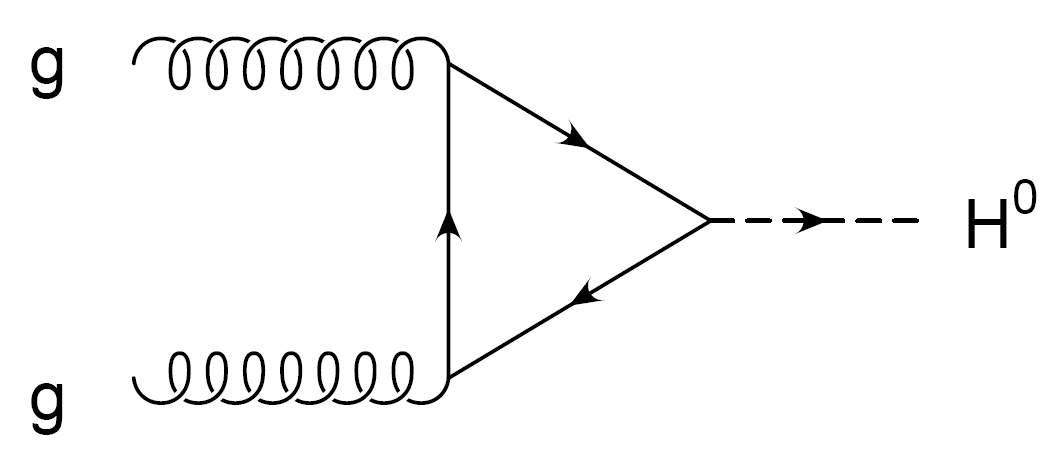
\includegraphics[width=0.4\textwidth]{images/gluon_fusion.png}}
 \subfigure[VBF]{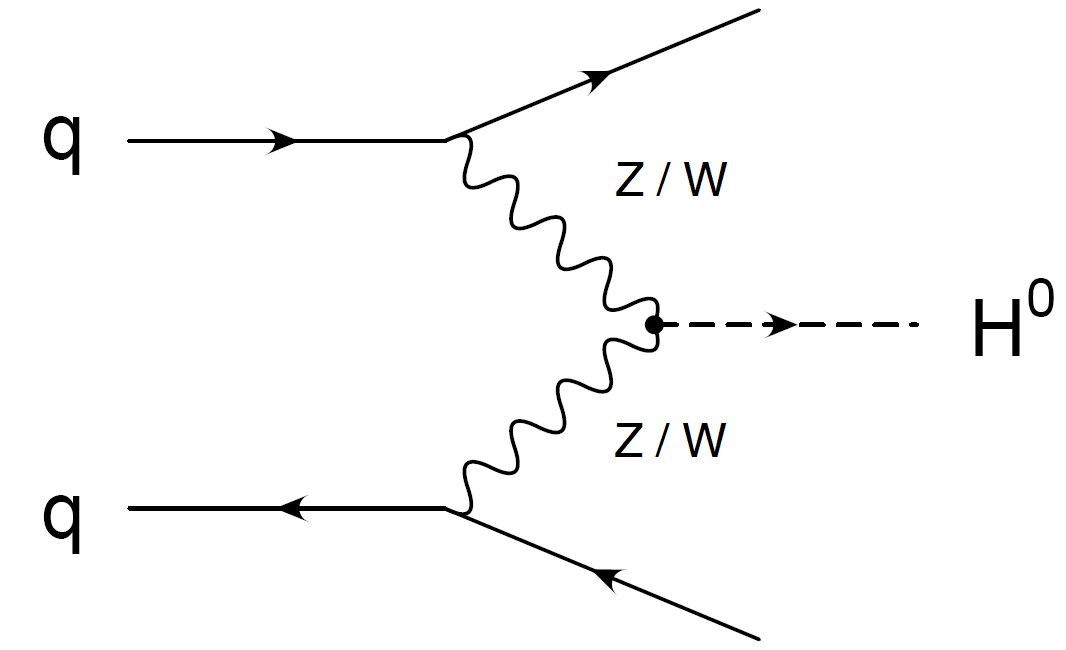
\includegraphics[width=0.3\textwidth]{images/vector_boson_fusion.png}}
 \caption{Feynmann diagrams of the two main production mechanisms for X.\label{fig:prod}}
\end{figure}

The details and precise meaning of the Feynman dagrams of Fig.~\ref{fig:prod}
are not relevant for this exercise, the relevant piece of information is that
two mechanisms are available and that they are marked by a substantial
difference: {\bf the ggF shows no other particles in the final state beyond X,
the VBF has two quarks in addition to the X in the final state}.
Although it should be noted that a precise calculation shows that additianal
particles in the form of hadronic jets can also arise in ggF, it remains true
that events arising from the two mechanisms are different when it comes to the
number of jets produced in addition to the X particle.

The production cross section for the Higgs boson as a function of its mass is
reported in Fig.~\ref{fig:production}. Although we now know the mass of the
Higgs boson to be 125 GeV, this plot is useful because it can be used as a
model for the expected cross section for X.
\begin{figure}
 \centering 
 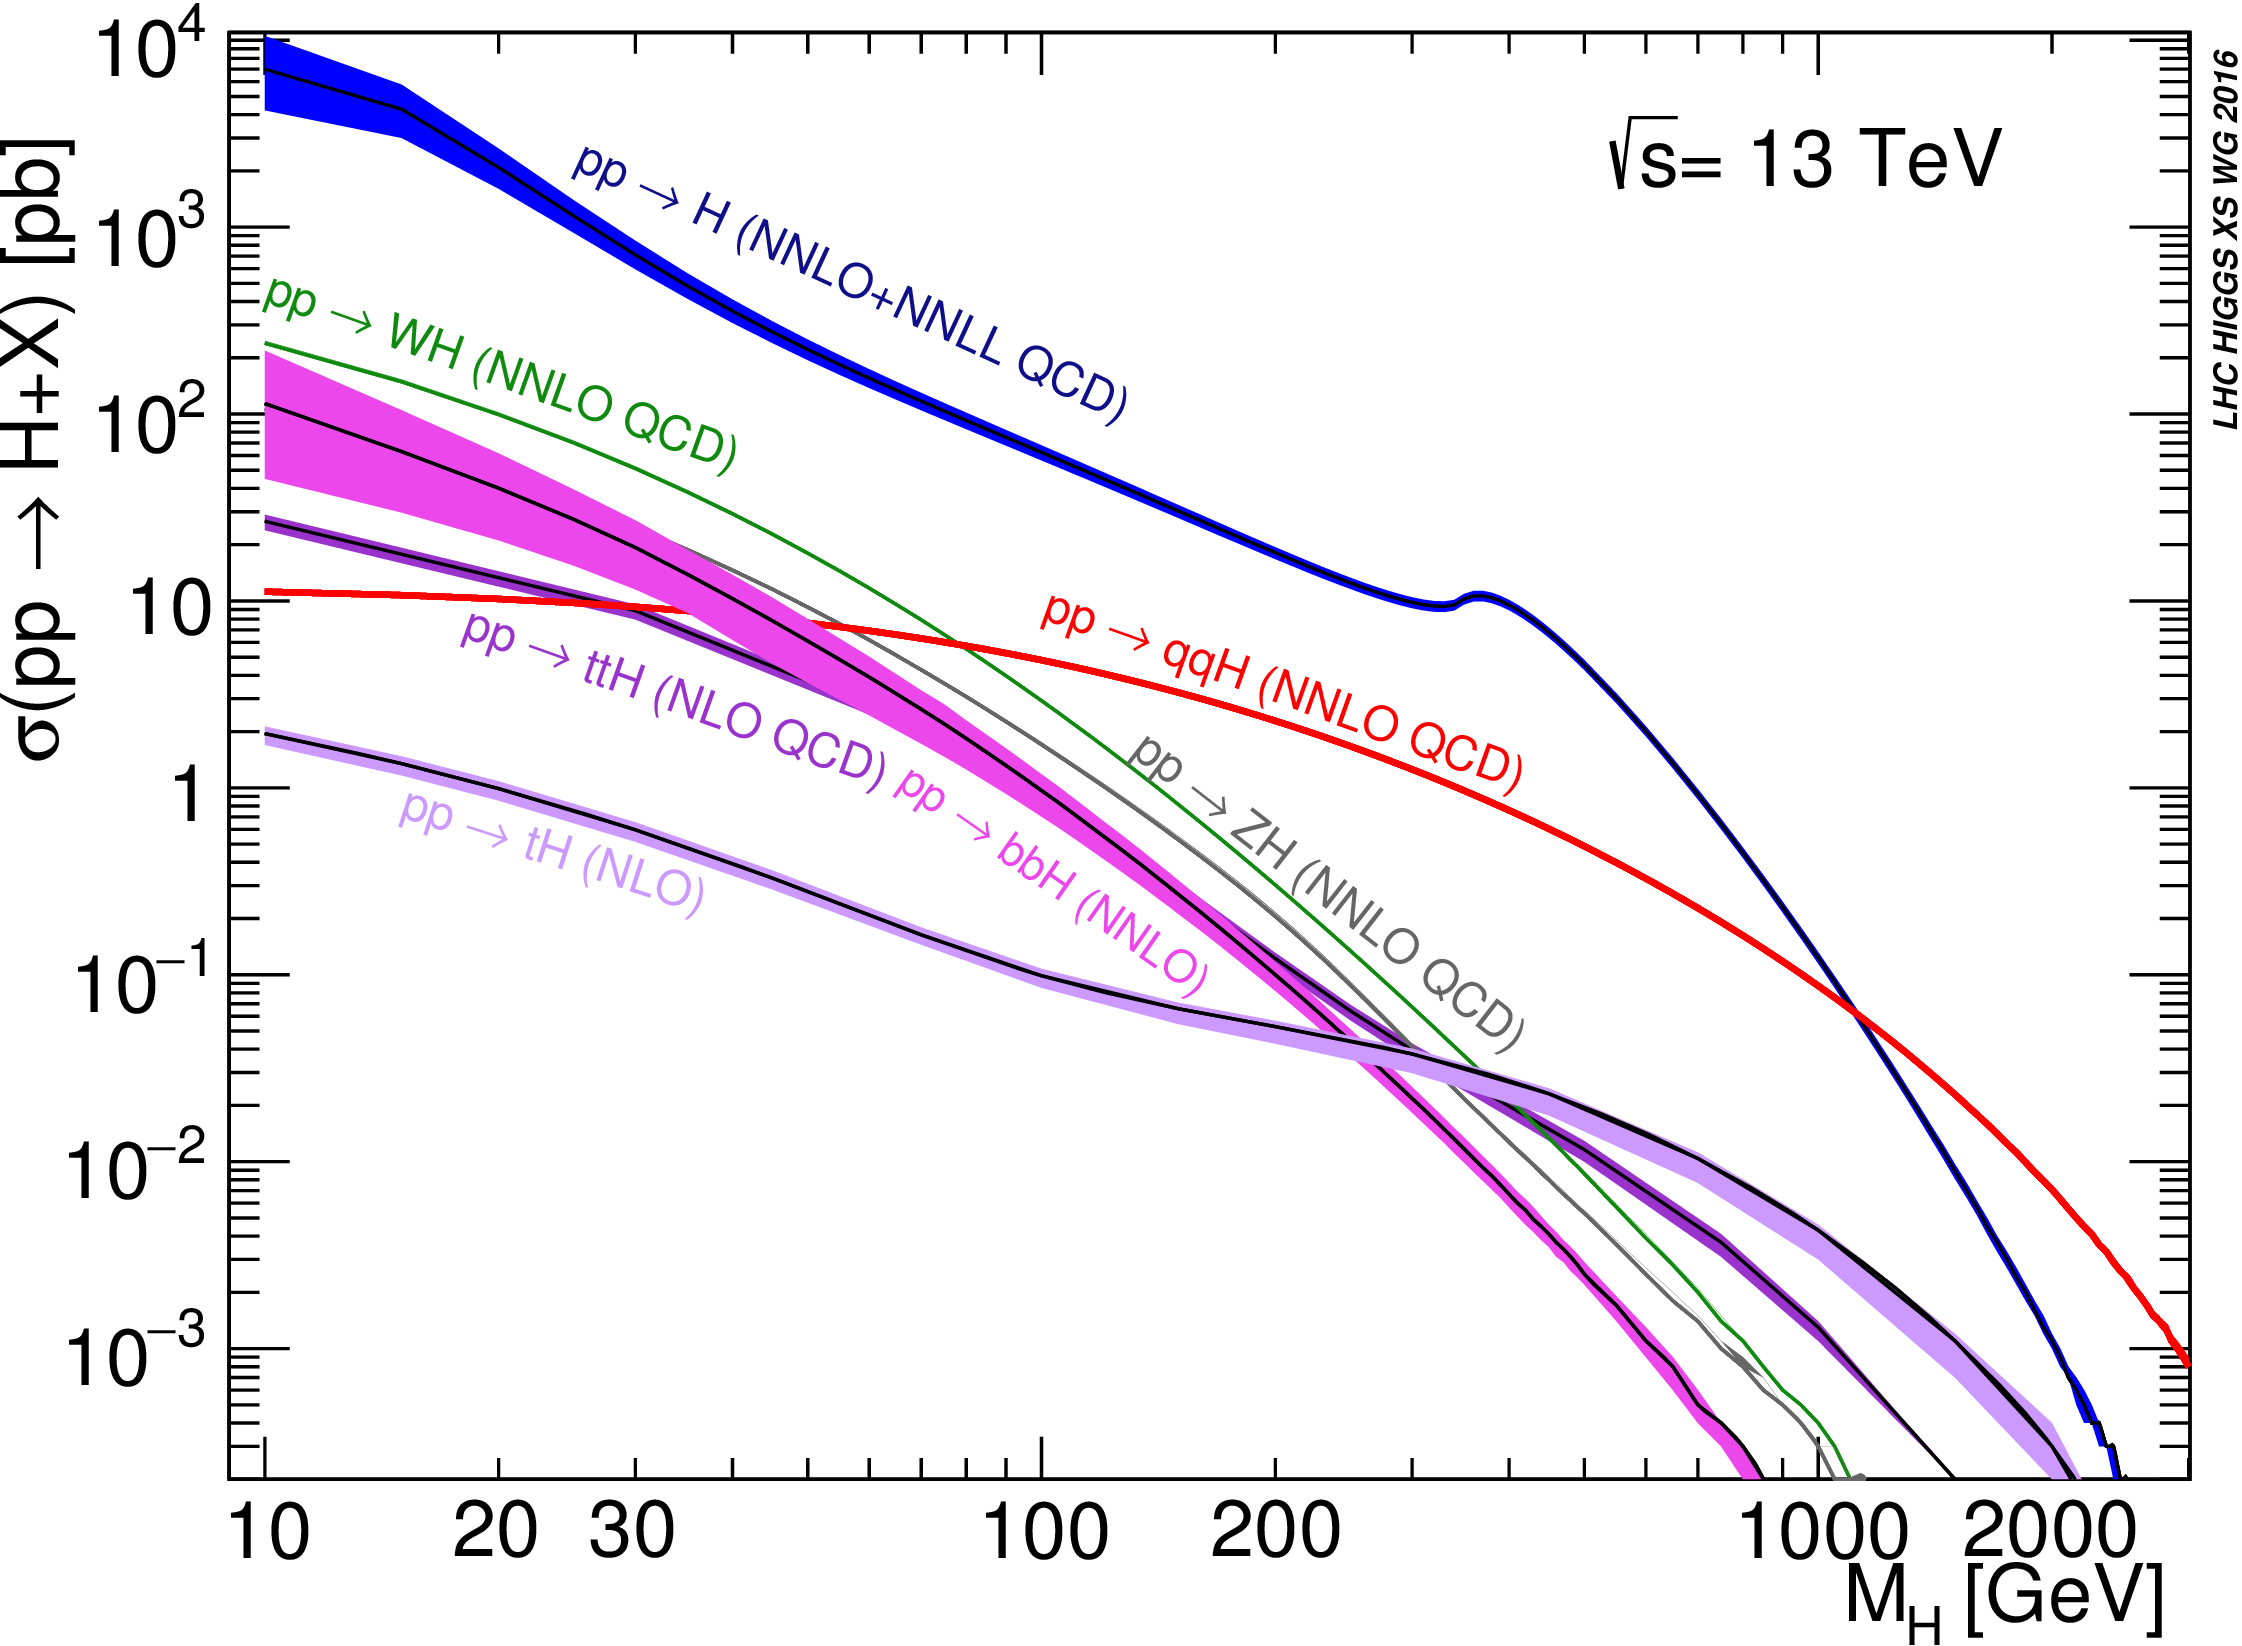
\includegraphics[width=0.5\textwidth]{images/plotAll_13tev_BSM_sqrt.png}
 \caption{Standard model Higgs boson cross section as a function of the mass
 of the Higgs boson. The ggF mechanisms is labeled $pp\rightarrow{}H$, the VBF
 mechanism is labeled $pp\rightarrow{}qqH$. Also other, sub-leading mechanisms
 are reported, which we will neglect.\label{fig:production}}
\end{figure}

We will assume that the cross section $\sigma$ for each of the production
channels of X scales with a common factor $\mu$ of the corresponding Higgs
boson cross section: \begin{equation}
 \sigma_{X [ggF,VBF]}(M) = \mu(M)\sigma_{H [ggF,VBF]}(M)
\end{equation}
 where M is the mass of X, and obvious meaning of the other symbols. This is a
 reasonable assumption, verified by several new physics models.  We notice
 that {\bf the relative importance of the VBF mechansm grows with the X mass},
 and becomes dominant above \~1.5 TeV.
 
 We will assume that, like H, also X has several decay channels. We assume
 that X has the same branching ratios of H, which are summarized in
 Fig.~\ref{fig:br}.  \begin{figure}
 \centering 
 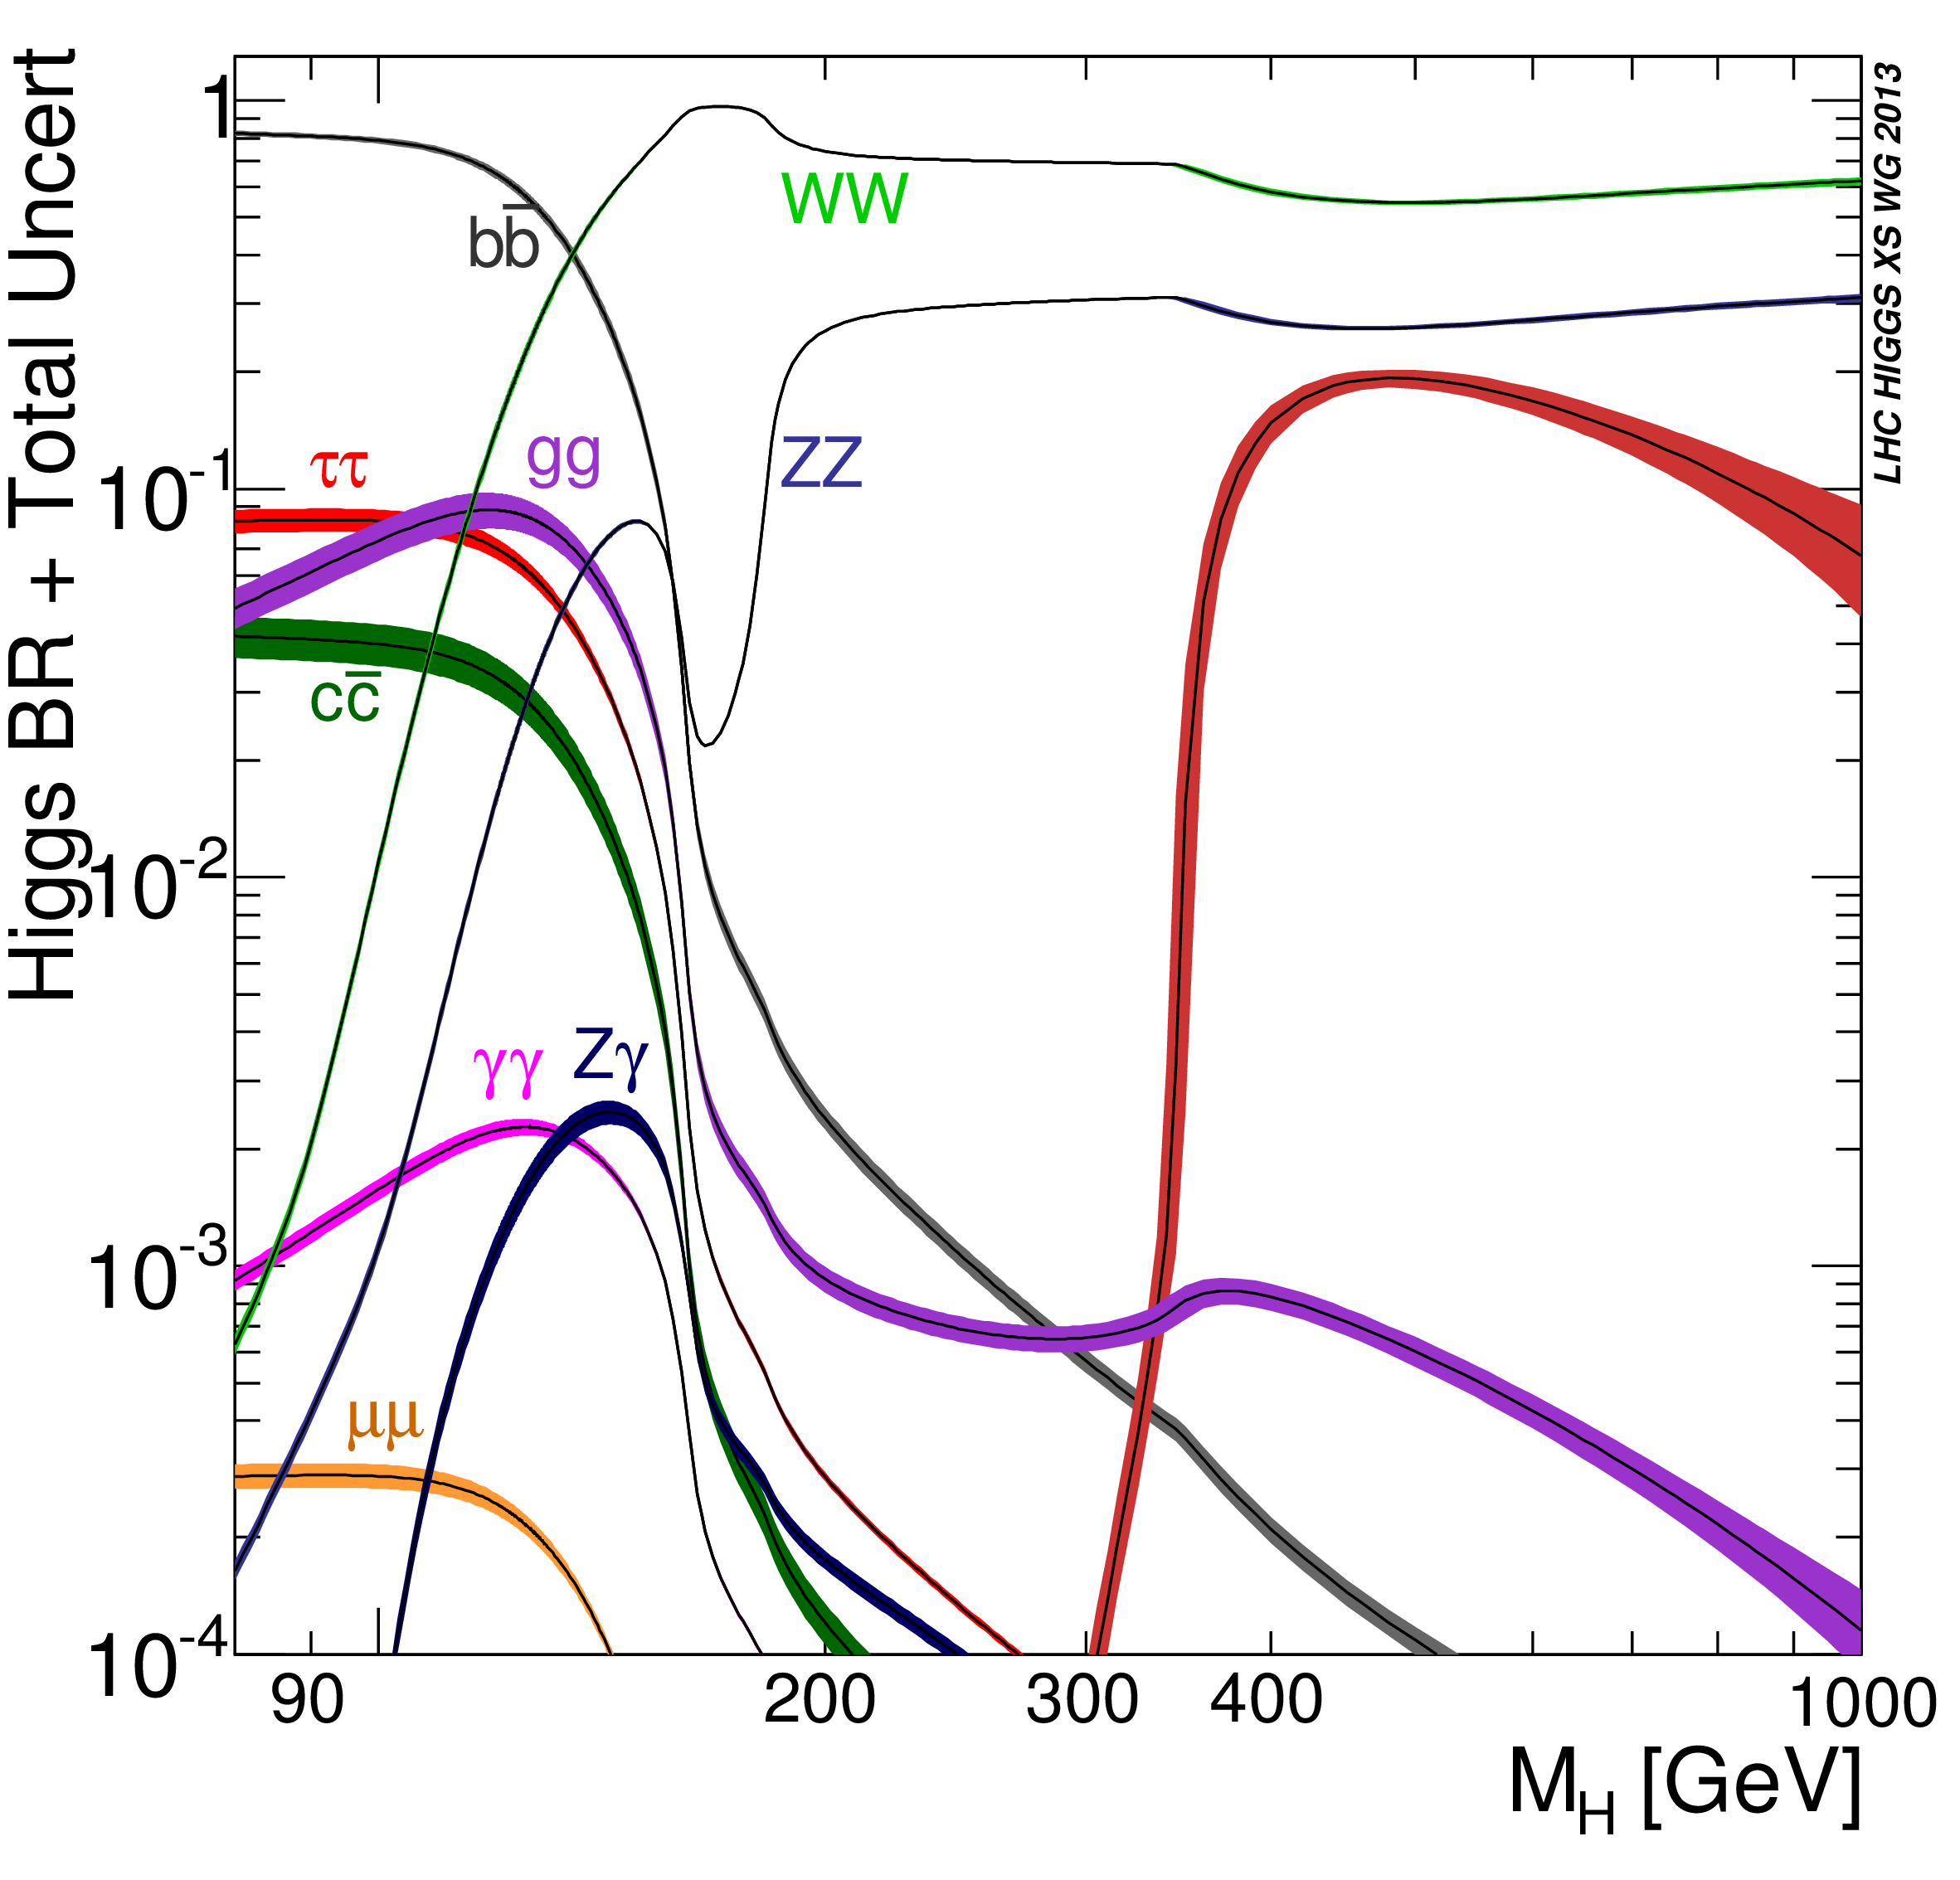
\includegraphics[width=0.5\textwidth]{images/Higgs_BR.png}
 \caption{Standard model Higgs boson cross section as a function of the mass
 of the Higgs boson. The ggF mechanisms is labeled $pp\rightarrow{}H$, the VBF
 mechanism is labeled $pp\rightarrow{}qqH$. Also other, sub-leading mechanisms
 are reported, but we will neglect them.\label{fig:br}}
\end{figure}
It should be noted that {\bf the WW decay channel is the one with the highest
branching ratio}.

\section{Data sample and analysis strategy}
Owing to the large branching fraction in the WW final state we choose this
channel for our search. In other words we search for the decay
X$\rightarrow$WW. The W bosons are themselves unstable and can decay
to a charged lepton (electron, muon, tauon) and a neutrino (30\% of the times
overall, equally divided for the three lepton species) and 70\% to a pair of
hadrons. In this exercise we will concentrate on the leptonic decays of the W
bosons. The reason of this choice will become clearer in when we discuss
backgrounds, but let us mention already that requiring leptons in the final
state allows a dramatic reduction of background processes. 
To summarise, {\bf we search for the H$\rightarrow$WW$\rightarrow{}2l2\nu$ decay
chain}.

We will use data collected by the CMS experiment in the 2015 data taking at
the LHC. These data correspond to an integrated luminosity of 2.3~fb$^{-1}$.
We will base our analysis on data reconstructed with the official CMS software
and Simulations for both the signal and the background processes. These data
come in the form of ROOT trees.

For each event the tree stores several event variables, in particular:
\begin{itemize}
\item[-] reconstructed leptons kinematic variables;
\item[-] the reconstructed missing transverse energy;
\item[-] the reconstructed jet kinematic variables.
\item[-] several weights, used both to improve the Data/Simulation agreement
and to normalize the simulation to the data luminosity.
\end{itemize}

\subsection{Main backgrounds}
A background process in a high energy physics analysis is a physics process
that yields a final state that resembles that of the signal.
In the case of this analysis there are two main background processes:
\begin{itemize}
\item production of two W bosons without an intermediate X;
\item production of a pair of top quarks, $t\bar{t}$. The top quark decays to
a b quark and a W boson.
\end{itemize}
The Feynman diagrams of these two processes are reported in
Fig.~\ref{fig:backgrounds} for the interested reader.

\begin{figure}
\centering
\subfigure{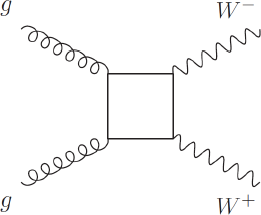
\includegraphics[width=0.3\textwidth]{images/ggWW.png}}
\subfigure{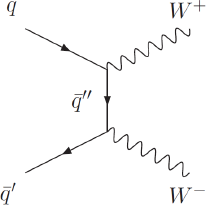
\includegraphics[width=0.3\textwidth]{images/qqWW.png}}
\subfigure{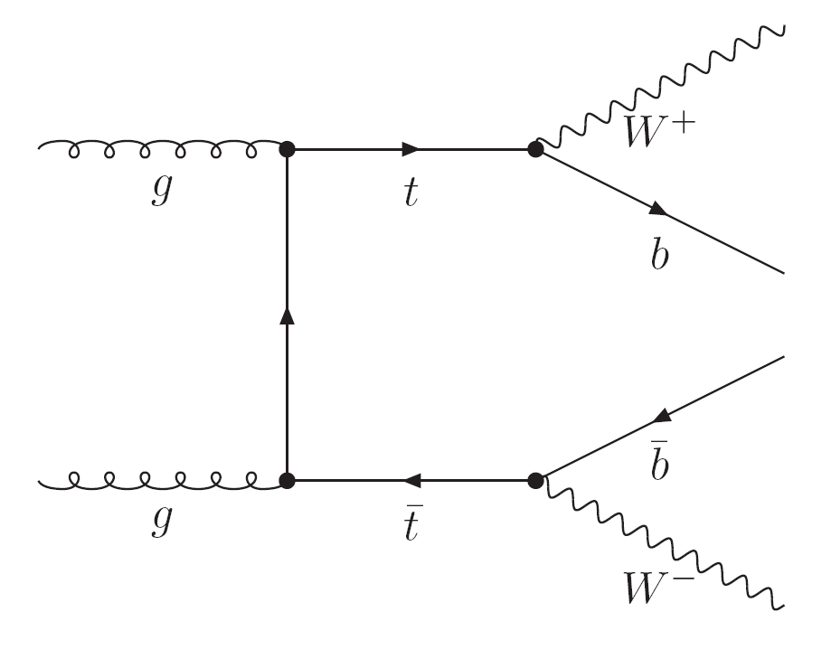
\includegraphics[width=0.3\textwidth]{images/ggtt.png}}
\caption{Gluon initiated (a) and quark initiated (b) WW. Top pair production
(c).\label{fig:backgrounds}}
\end{figure}

We apply a series of cuts to reduce their contribution as much as possible.
$t\bar{t}$ is reduced by requiring that jets in the event are not compatible
with being originated from b quarks, using dedicated jet-tagging techniques.
WW is reduced with kinematic cuts on the leptons.

Other subleading sources of background originate from processes in which at
least one of the leptons is not a real lepton, but is identified as such by the
reconstruction algorithms. The control of these backgrounds is a crucial part of the analysis,
but is beyond the scope of this exercise. The cuts to be applied will be
provided by the teachers.

\subsection{Main discriminating variable}
After the selection cuts mentioned above to suppress the backgrounds we end up
with a sample that is primarily composed of WW and $t\bar{t}$. In order to
further discriminate a possible signal and backgrounds we use a kinematic
variable called $m_{T,i}$. This variable is the invariant mass of the
4-momentum resulting from the sum of the two lepton 4-momenta and the MET
4-momentum. Since we are unable to reconstruct the longitudinal component of
the neutrinos momenta, this variable is the closest approximation of
the resonance invariant mass that we can in a signal event, and it retains a
significant discriminating power with respect to backgrounds.

The distribution of  $m_{T,i}$ is shown in Fig.~\ref{fig:mti} after the
selection cuts. The data point are show on top of the stack of the
backgrounds. The shape of a signal for X mass of 1 TeV is also shown
(multiplied by 10). The rightmost bin of each distribution is an overflow bin.
The fact that the signal shape does not peak at 1 TeV is due to 
$m_{T,i}$ lacking the contribution from the longitudinal  momenta of neutrinos.
\begin{figure}[!b]
\centering
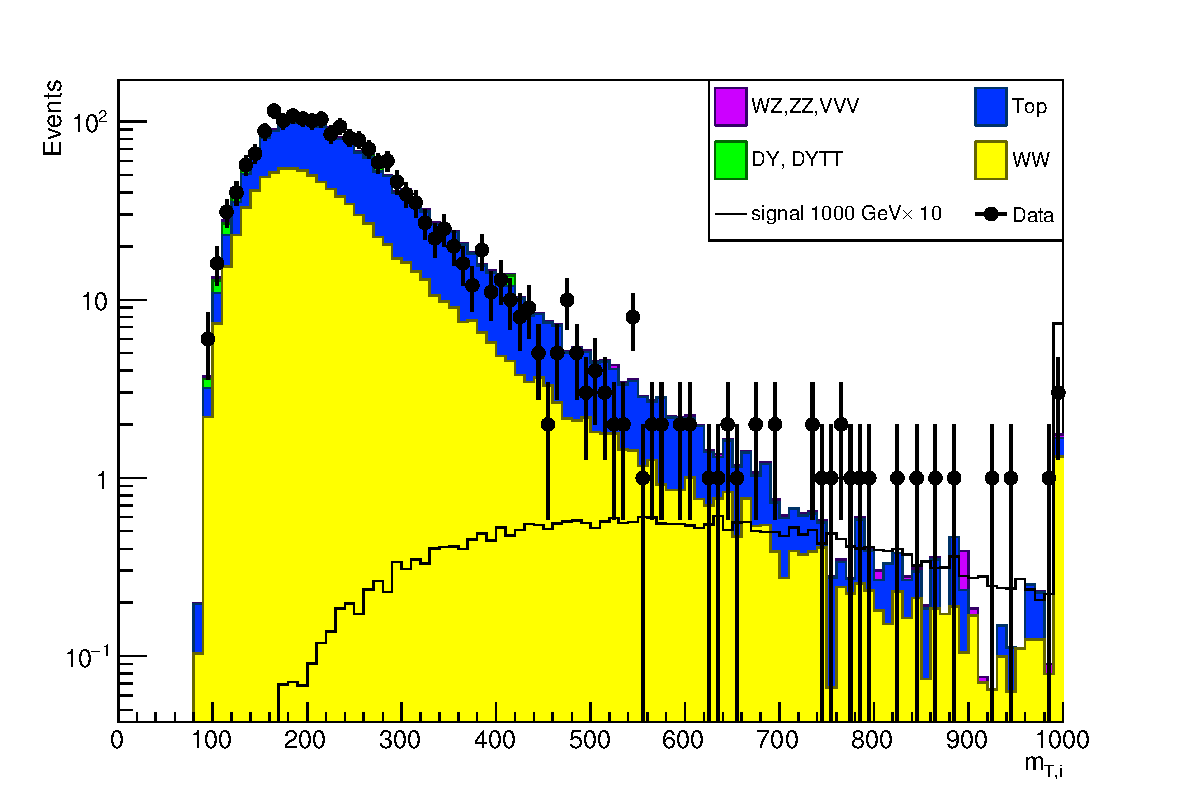
\includegraphics[width=0.6\textwidth]{images/mTi.pdf}
\caption{$m_{T,i}$ in data and simulation for 2015 data after selection cuts.\label{fig:mti}}
\end{figure}

\subsection*{Exercise 1: }
{\bf Write a code that builds the stack of backgrounds to obtain a plot
similar to Fig.~\ref{fig:mti}.}

A set of root files is provided, together with a root macro
(\verb;HWWYields.C;) implementing selection cuts.

Each root file contains a root tree names \verb;latino;. This tree holds
several variables, including $m_{T,i}$ in a branch called \verb;mTi;.

Eight data files are provided, corresponding to two distinct data taking periods
(called \verb;Run2015C; and \verb;Run2015D;) and four triggers. Data from CMS
are in fact divided into different streams depending on the triggers each
event fires. In this analysis we use events with at least two electrons
(\verb;DoubleEG;), at least two muons (\verb;DoubleMu;), at least an electron and a muon
(\verb;MuonEG;) or at least a muon  (\verb;SingleMuon;). The latter is used
only to recover an inefficiency in the other triggers.

Simulated events (MC) are produced for several physics processes, including
$t\bar{t}$, WW, Z$\rightarrow{}\tau\tau$, and other subleading processes.
Simulated samples for different mass hypotheses for X are also provided. For
each mass hypothesis two different files are provided, one containing the
simulation of the ggF production mechanism and the other containing the
simulation for the VBF production mechanism.

\subsection{Cut based analysis}

\end{document}          
